\documentclass[a4paper,10pt]{article}
\usepackage[utf8]{inputenc}
\usepackage[slovene]{babel}
\usepackage{graphicx}
\usepackage{hyperref}
\usepackage[left=2cm,right=2cm,top=2cm,bottom=3cm]{geometry}
\usepackage{amsmath}
\usepackage{float}
\usepackage{bbold}

\makeatletter
\renewcommand*\env@matrix[1][*\c@MaxMatrixCols c]{%
  \hskip -\arraycolsep
  \let\@ifnextchar\new@ifnextchar
  \array{#1}}
\makeatother

%opening
\title{Modelekularna dinamika}
\author{Miha \v Can\v cula}

\newcommand{\uvec}[1]{\ensuremath{\underline{#1}}}
\newcommand{\bb}{
  \ensuremath{b_1 b_2 \ldots b_n}
}
\newcommand{\psibb}{
  \ensuremath{\psi_{\bb}}
}

\begin{document}

\maketitle

\section{Transport toplote}

Transport toplote sem preu"ceval z enodimenzionalno verigo oscilatorjev. 
Delca na konceh verige sem sklopil s toplotnima kopelima z brezdimenzijskima temperaturama $T_L=1$ in $T_R=2$. 

Zanimajo nas vrednosti v stacionarnem stanju, zato sem najprej napravil $N_I = 10^{8}$ korakov integracije dol"zine $h=10^{-2}$. 
Nato sem izvedel "se $N_A=10^{7}$ korakov, med katerimi sem opravil $10^{5}$ meritev temperature in toplotnega toka. 
Meritve sem na koncu popre"cil. 

\section{Maxwellske kopeli}

Najprej sem za modeliranje toplotnih kopeli uporabil Maxwellov algoritem, pri katerem gibalni koli"cini sklopljenih delcev resetiramo vsakih $R=100$ korakov. 
Preizku"sal sem razli"cne vrednosti za $R$, najbolje pa se je izkazala tak"sna, pri kateri se reset zgodi enkrat vsako "casovno enoto, torej $Rh \sim 1$. 
Med reseti sem stanje propagiral s simplekti"cnim integratorjem s simetri"cno shemo $S_2$. 

\input{g_odv_lambda_30}

\input{g_odv_lambda_100}

\input{g_odv_velikost}

% GNUPLOT: LaTeX picture with Postscript
\begingroup
  \makeatletter
  \providecommand\color[2][]{%
    \GenericError{(gnuplot) \space\space\space\@spaces}{%
      Package color not loaded in conjunction with
      terminal option `colourtext'%
    }{See the gnuplot documentation for explanation.%
    }{Either use 'blacktext' in gnuplot or load the package
      color.sty in LaTeX.}%
    \renewcommand\color[2][]{}%
  }%
  \providecommand\includegraphics[2][]{%
    \GenericError{(gnuplot) \space\space\space\@spaces}{%
      Package graphicx or graphics not loaded%
    }{See the gnuplot documentation for explanation.%
    }{The gnuplot epslatex terminal needs graphicx.sty or graphics.sty.}%
    \renewcommand\includegraphics[2][]{}%
  }%
  \providecommand\rotatebox[2]{#2}%
  \@ifundefined{ifGPcolor}{%
    \newif\ifGPcolor
    \GPcolortrue
  }{}%
  \@ifundefined{ifGPblacktext}{%
    \newif\ifGPblacktext
    \GPblacktexttrue
  }{}%
  % define a \g@addto@macro without @ in the name:
  \let\gplgaddtomacro\g@addto@macro
  % define empty templates for all commands taking text:
  \gdef\gplbacktext{}%
  \gdef\gplfronttext{}%
  \makeatother
  \ifGPblacktext
    % no textcolor at all
    \def\colorrgb#1{}%
    \def\colorgray#1{}%
  \else
    % gray or color?
    \ifGPcolor
      \def\colorrgb#1{\color[rgb]{#1}}%
      \def\colorgray#1{\color[gray]{#1}}%
      \expandafter\def\csname LTw\endcsname{\color{white}}%
      \expandafter\def\csname LTb\endcsname{\color{black}}%
      \expandafter\def\csname LTa\endcsname{\color{black}}%
      \expandafter\def\csname LT0\endcsname{\color[rgb]{1,0,0}}%
      \expandafter\def\csname LT1\endcsname{\color[rgb]{0,1,0}}%
      \expandafter\def\csname LT2\endcsname{\color[rgb]{0,0,1}}%
      \expandafter\def\csname LT3\endcsname{\color[rgb]{1,0,1}}%
      \expandafter\def\csname LT4\endcsname{\color[rgb]{0,1,1}}%
      \expandafter\def\csname LT5\endcsname{\color[rgb]{1,1,0}}%
      \expandafter\def\csname LT6\endcsname{\color[rgb]{0,0,0}}%
      \expandafter\def\csname LT7\endcsname{\color[rgb]{1,0.3,0}}%
      \expandafter\def\csname LT8\endcsname{\color[rgb]{0.5,0.5,0.5}}%
    \else
      % gray
      \def\colorrgb#1{\color{black}}%
      \def\colorgray#1{\color[gray]{#1}}%
      \expandafter\def\csname LTw\endcsname{\color{white}}%
      \expandafter\def\csname LTb\endcsname{\color{black}}%
      \expandafter\def\csname LTa\endcsname{\color{black}}%
      \expandafter\def\csname LT0\endcsname{\color{black}}%
      \expandafter\def\csname LT1\endcsname{\color{black}}%
      \expandafter\def\csname LT2\endcsname{\color{black}}%
      \expandafter\def\csname LT3\endcsname{\color{black}}%
      \expandafter\def\csname LT4\endcsname{\color{black}}%
      \expandafter\def\csname LT5\endcsname{\color{black}}%
      \expandafter\def\csname LT6\endcsname{\color{black}}%
      \expandafter\def\csname LT7\endcsname{\color{black}}%
      \expandafter\def\csname LT8\endcsname{\color{black}}%
    \fi
  \fi
  \setlength{\unitlength}{0.0500bp}%
  \begin{picture}(7200.00,5040.00)%
    \gplgaddtomacro\gplbacktext{%
      \csname LTb\endcsname%
      \put(1078,704){\makebox(0,0)[r]{\strut{} 1.3}}%
      \put(1078,1518){\makebox(0,0)[r]{\strut{} 1.35}}%
      \put(1078,2332){\makebox(0,0)[r]{\strut{} 1.4}}%
      \put(1078,3147){\makebox(0,0)[r]{\strut{} 1.45}}%
      \put(1078,3961){\makebox(0,0)[r]{\strut{} 1.5}}%
      \put(1078,4775){\makebox(0,0)[r]{\strut{} 1.55}}%
      \put(1210,484){\makebox(0,0){\strut{} 0}}%
      \put(1909,484){\makebox(0,0){\strut{} 0.02}}%
      \put(2608,484){\makebox(0,0){\strut{} 0.04}}%
      \put(3307,484){\makebox(0,0){\strut{} 0.06}}%
      \put(4007,484){\makebox(0,0){\strut{} 0.08}}%
      \put(4706,484){\makebox(0,0){\strut{} 0.1}}%
      \put(5405,484){\makebox(0,0){\strut{} 0.12}}%
      \put(6104,484){\makebox(0,0){\strut{} 0.14}}%
      \put(6803,484){\makebox(0,0){\strut{} 0.16}}%
      \put(176,2739){\rotatebox{-270}{\makebox(0,0){\strut{}$T(1/5)$}}}%
      \put(4006,154){\makebox(0,0){\strut{}$\lambda$}}%
    }%
    \gplgaddtomacro\gplfronttext{%
      \csname LTb\endcsname%
      \put(2266,1977){\makebox(0,0)[r]{\strut{}$N = 10$}}%
      \csname LTb\endcsname%
      \put(2266,1757){\makebox(0,0)[r]{\strut{}$N = 20$}}%
      \csname LTb\endcsname%
      \put(2266,1537){\makebox(0,0)[r]{\strut{}$N = 30$}}%
      \csname LTb\endcsname%
      \put(2266,1317){\makebox(0,0)[r]{\strut{}$N = 50$}}%
      \csname LTb\endcsname%
      \put(2266,1097){\makebox(0,0)[r]{\strut{}$N = 100$}}%
      \csname LTb\endcsname%
      \put(2266,877){\makebox(0,0)[r]{\strut{}$N = 200$}}%
    }%
    \gplbacktext
    \put(0,0){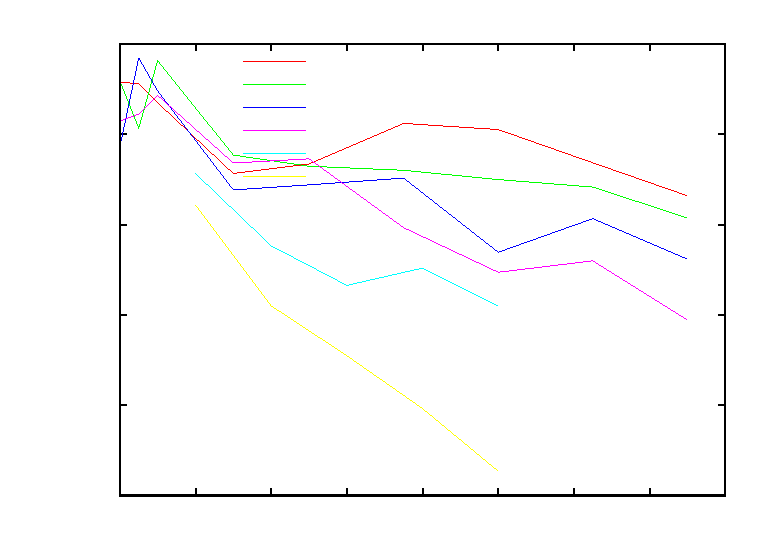
\includegraphics{g_prehod}}%
    \gplfronttext
  \end{picture}%
\endgroup


\section{Nos\'e-Hooverjeve kopeli}

\end{document}
